\section{Arcjets}

\subsection{Principles}

Arcjets constitute a branch of propulsion technology under the electrothermal electrical rocket propulsion heading. AS such, to generate thrust, the propellant is heated and forced trough a typical convergent-divergent nozzle. Heat is transferred to the propellant using an electric arc induced by a high current discharge. As stated in \cite{rpe_book}, the physical components of the system are relatively simple, as opposed to the phenomenology they explore: \textit{plasma physics}. The electric effect requires cathode and anode elements. These requirements are solved by typically placing the cathode as a centered element inside the nozzle, with the nozzle shell serving itself as the anode element.

\begin{figure}[h]
    \centering
    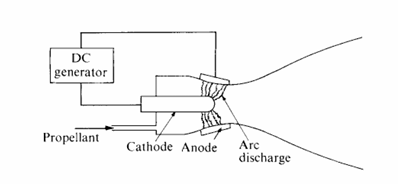
\includegraphics[width=0.5\linewidth]{figs/arcjet_pic1.png}
    \caption{Schematic diagram of an arcjet \cite{mtp_book}}
    \label{arcjet_schematics}
\end{figure}

The largest differentiator of this technology is the ability to achieve heating temperatures much higher than surrounding walls, overcoming the fundamental limitation of \textit{Resistojet Rocket Propulsion} systems.


\subsection{Electric Subsystem}

All the arcjet working architecture assume the successful generation of an electric arc. As the propellants, in the chamber, are a gaseous medium, electricity conduction trough it requires that a certain ionization threshold is achieved. This effect is analogous to a lightning discharge. Overall, this process is inherently unstable, \cite{agr_book}, thus consisting in the most difficult stage of arcjet propulsion systems. To stabilize the electrical arc, a constrictor design  with tangential propellant injection is often employed, to induce a swirl inside the nozzle. This also helps with cooling and preserving the nozzle material. \cite{pep_book}

A sensible approach for the plasma physics is to consider the gaseous medium as uniform. Applying the generalized Ohm's Law, the propellant is subject to Ohmic heating. \cite{rpe_book}

\begin{equation}
\label{eq:ohm_1}
    V = IR = \left( \frac{I}{A} \right) \left( \frac{AR}{d} \right) (d)
\end{equation}

Equation \eqref{eq:ohm_1} assuming the very same uniform medium, the electric field is $E = V / d$, current density $j = I/A$ and \textit{electrical conductivity} as $\sigma = d / AR$. The electrical conductivity is proportional to \textit{free electrons} \cite{rpe_book}. 

The ionization level useful to the process depends on: High temperatures and/or low ionization threshold requirements. To help kickstart the effect, the gases may be pre-processed by \textit{seeding} them with low ionization potential vapors. The plasma conductivity can be calculated regarding the free electrons motion.


\begin{equation}
\label{eq:sigma_condut}
    \sigma = \frac{e^2n_e\tau}{\mu_e} 
\end{equation}

In reality, arc currents are influenced by magnetic fields,  further detailed models exist to represent the phenomena. \cite{rpe_book}. If constant conductivity $\sigma$ si assumed, the volumetric power input can be computed as \cite{pep_book}:

\begin{equation}
\label{eq:arcjet_pele_comp}
    P_e = j \cdot E = \sigma E^2
\end{equation}

To start and arcjet thruster, an initial higher voltage discharge is employed to disrupt the cold gas and induce plasma production. After that, the steady-state arc is preserved and conditioned with resistance or ballast mechanism. \cite{rpe_book}

Downstream the arc, the propellant is partially ionized into a plasma, a enthalpy rich state, of mainly thermal and ionization energy. The further expansion over the nozzle provides the conversion into the desired kinetic energy.

\subsection{Mathematical Model}

As stated in the previous chapter, arcjet modeling requires the coupling of both fluid dynamics and electromagnetic principles.

Narrowing down the envelope of operation to free space (vacuum), thrust can be derived from the momentum balance of the nozzle outer boundary:

\begin{equation}
\label{eq:arcjet_thrust}
    F = \dot{m} u_e
\end{equation}

With specific impulse:

\begin{equation}
\label{eq:isp_arcjet}
    I_{sp} = \frac{u_e}{g_0} =\frac{F}{\dot{m} g_0}
\end{equation}

Thruster efficiency is given by the ratio between the power of jet and the power input:

\begin{equation}
\label{eq:arcjet_eff_1}
    \eta_T = \frac{power \ of \ the \ jet}{overall \ power \ input}
\end{equation}

Depending on the propellant used and system architecture, the input power may be all electrical, or a combination of electrical and chemical energy, as in hydrazine decomposition \cite{rpe_book}. With $P_e = electric \ power$,generalized ohms law, $P_{chem} = chemical \ power$ and $P_{in} = power \ input$:

\begin{equation}
\label{eq:pchm_arcjet}
    P_{chem} = \dot{m} \ h_{chem}
\end{equation}

\begin{equation}
\label{eq:pi_arcjet}
    P_{in} = P_e + P_{chem} 
\end{equation}

The power generated on the thruster results from the kinetic energy rate seen at the nozzle exhaust \cite{rpe_book}: 

\begin{equation}
\label{eq:pj_arcjet}
    P_{j} = \frac{1}{2} \dot{m} u_e^2 =  \frac{1}{2} \dot{m} \left( \frac{F}{\dot{m}} \right)^2 = \frac{F^2}{2 \dot{m}}
\end{equation}

Replacing \eqref{eq:pj_arcjet} and \eqref{eq:pi_arcjet} into \eqref{eq:arcjet_eff_1}:

\begin{equation}
\label{eq:arcjet_eff_2}
    \eta_t = \frac{P_j}{P_{in}} = \frac{\frac{1}{2} \dot{m}u_e^2}{P_e + P_{chem}} = \frac{\frac{1}{2} \frac{F}{I_{sp} g_0} \left( I_{sp} g_0 \right)^2}{P_e + P_{chem}} = \frac{1}{2} \frac{F I_{sp} g_0}{{P_e + P_{chem}}}
\end{equation}

For scenarios where chemical energy is meaningless, the efficiency if further simplified into:

\begin{equation}
\label{eq:arcjet_eff_3}
    \eta_t = \frac{F I_{sp} g_0}{2 P_e}
\end{equation}

Combining $P_j$ with $P_in$, $\eta_t$ and $I_{sp}=$ \cite{fep_book}, the system can be expressed as $u_e$ \eqref{eq:arcjet_ue} or $I_{sp}$ \eqref{eq:arcjet_isp}:

\begin{equation}
\label{eq:arcjet_ue}
    \eta_t = \frac{\frac{1}{2} \dot{m}u_e^2}{P_{in}} \Leftrightarrow u_e = \sqrt{\frac{2 \eta_t P_e}{\dot{m}}} 
\end{equation}


\begin{equation}
\label{eq:arcjet_isp}
    \eta_t = \frac{\frac{1}{2} \dot{m}u_e^2}{P_{in}} \Leftrightarrow u_e = \sqrt{\frac{2 \eta_t P_e}{\dot{m}}} \Leftrightarrow I_{sp} = \frac{1}{g_0} \sqrt{\frac{2 \eta_t P_e}{\dot{m}}}
\end{equation}

\subsection{Specific Characteristics}

For current technology,  only roughly half of the energy can be converted into useful kinetic energy. Up to 20 \% is wasted as heat, via dissipation and radiation, with the remaining fraction representing the residual energy and ionization present on the plume. This effect, frozen flow, results from the dissociation of molecules due to the electric arc and inability to recombine in the nozzle due to the very fast flow.  At the same time, the cathode suffers erosion, aggravated by power cycling. This contributes to an additional loss of efficiency over the lifespan of the thruster.\cite{mtp_book}


%\begin{table}[H]
%\centering
%\caption{Typical Performance Parameters of Arcjet Propulsion Systems \cite{rpe_book}}
%\label{tab:arcjet_performance}
%\begin{tabular}{@{}ll@{}}
%\toprule
%\textbf{Parameter} & \textbf{Typical Value} \\ \midrule
%Thrust Range (mN) & 200 -- 1000 \\
%Specific Impulse (sec) & 400 -- 800 \\
%Thruster Efficiency (\%) & 30 -- 50 \\
%Thrust Duration & Months \\
%Typical Propellants & $H_2$, $N_2$, $N_2H_4$, $NH_3$ \\
%Kinetic Power per Unit Thrust (W/mN) & 2-3 \\ \bottomrule
%\end{tabular}
%\end{table}
